\chapter{Vers l'étude des simulations Landau-fluides}
\renewcommand\partie{\Partie\ Chapitre \thechapter}
\label{ch-34}

\bigskip
\minitoc  

\cite{ferrand_fluid_2021} ont aussi utilisé des simulations du modèle \acs{LFHPe} prenant en compte un flux de chaleur $\overline{\overline{\boldsymbol{q}}}$ gyrotrope obtenu grâce à une fermeture Landau-fluide présente dans le code utilisé dans cette partie. Il s'est avéré que ces simulations prennent aussi en compte un tenseur de pression électronique de type gyrotrope.
Ces simulations corrigeant les critères d'instabilités tel que le critère miroir afin de refléter le comportement linéaire cinétique, elles pourraient par la suite nous aider à étendre nos interprétations vers les processus cinétiques. 

Dans ce chapitre, nous décrivons les spécificités du modèle implémenté et la loi exacte complète associée. Une première application, préliminaire, à deux simulations, semblent montrer des résultats paradoxaux qui nécessiteront une étude plus fine avant d'en extraire un début d'interprétations. 


\section{Modèle simulé et loi exacte}
\label{sec-341}

Dans ce deuxième lot de simulations, les ions et les électrons sont décrits avec un tenseur de pression gyrotrope. La fermeture utilisée est une fermeture Landau-fluide. Cette fermeture nous rapproche d'un modèle cinétique en prenant en compte l'amortissement Landau linéaire (phénomène cinétique) dans le modèle fluide. Cette correction étant basée sur la relation de dispersion cinétique, les critères d'instabilité seront aussi corrigés pour correspondre aux critères cinétiques. La gyrotropie des électrons impactera d'ailleurs le critère miroir. Les flux de chaleur ioniques et électroniques sont aussi supposés gyrotropes.

Les premières équations du modèle normalisé simulé sont les suivantes, en y faisant apparaître indépendamment les tenseurs de pression ionique et électronique : 
\begin{eqnarray}
\label{eq:mlf_r} \partial_t \rho + \nabla \cdot \left(\rho \boldsymbol{v}\right) &=& 0\\
\label{eq:mlf_v} \partial_t  \boldsymbol{v} + \boldsymbol{v} \cdot \nabla  \boldsymbol{v} - \frac{1}{\rho} \boldsymbol{j} \times \boldsymbol{B} + \frac{1}{\rho} \nabla \cdot \left(\overline{\boldsymbol{P_i}} + \overline{\boldsymbol{P_e}} \right)  &=& 0  \\
\label{eq:mlf_b} \partial_t \boldsymbol{B} - \nabla \times \left( \boldsymbol{v} \times \boldsymbol{B} \right) +  d_i  \nabla \times \left( \frac{1}{\rho} \boldsymbol{j}\times \boldsymbol{B} \right) &=& d_i \nabla \times \left( \frac{1}{\rho} \nabla \left(  p_e\right) \right)  \\
\label{eq:mlf_pperpi} \partial_t  p_{\perp i }  +  \nabla \cdot \left(p_{\perp i } \boldsymbol{v} \right) +  p_{\perp i }\nabla \cdot\boldsymbol{v} -  p_{\perp i } \boldsymbol{b}\boldsymbol{b} : \nabla \boldsymbol{v}  &=& - \frac{1}{2} \left( \text{Tr}(\nabla \cdot \overline{\overline{\boldsymbol{q_i}}}) - \boldsymbol{b}\boldsymbol{b} : \nabla \cdot \overline{\overline{\boldsymbol{q_i}}} \right) \nonumber \\ && \\
\label{eq:mlf_ppari} \partial_t  p_{\parallel i }  +  \nabla \cdot \left(p_{\parallel i } \boldsymbol{v} \right) +  2 p_{\parallel i }  \boldsymbol{b}\boldsymbol{b} : \nabla \boldsymbol{v}  &=&  - \boldsymbol{b}\boldsymbol{b} : \nabla \cdot \overline{\overline{\boldsymbol{q_i}}}   \\
\label{eq:mlf_pperpe} \partial_t  p_{\perp e }  +  \nabla \cdot \left(p_{\perp e } \boldsymbol{v_e} \right) +  p_{\perp e }\nabla \cdot\boldsymbol{v_e} -  p_{\perp e } \boldsymbol{b}\boldsymbol{b} : \nabla \boldsymbol{v_e}  &=&  - \frac{1}{2} \left( \text{Tr}(\nabla \cdot \overline{\overline{\boldsymbol{q_e}}}) - \boldsymbol{b}\boldsymbol{b} : \nabla \cdot \overline{\overline{\boldsymbol{q_e}}} \right) \nonumber \\ && \\
\label{eq:mlf_ppare} \partial_t  p_{\parallel e }  +  \nabla \cdot \left(p_{\parallel e } \boldsymbol{v_e} \right) +  2 p_{\parallel e }  \boldsymbol{b}\boldsymbol{b} : \nabla \boldsymbol{v_e}  &=& - \boldsymbol{b}\boldsymbol{b} : \nabla \cdot \overline{\overline{\boldsymbol{q_e}}} 
\end{eqnarray}

avec $\overline{\boldsymbol{P_{i,e}}} =  \frac{\beta_0}{2} \left(p_{\perp i,e } \overline{\boldsymbol{I}} + \left(p_{\parallel i,e } - p_{\perp i,e }\right) \boldsymbol{b} \boldsymbol{b} \right) $, les tenseurs gyrotropes de pression ionique (i) et électronique (e), $\boldsymbol{b} = \frac{\boldsymbol{B}}{|\boldsymbol{B}|}$, la direction du champ magnétique, $\frac{\beta_0}{2} $ constante provenant de la normalisation des équations, et $\boldsymbol{v_e} = \boldsymbol{v} - d_i \frac{\boldsymbol{j}}{\rho} $ la vitesse électronique. La fermeture est appliquée au niveau du quatrième moment (pour plus d'informations, voir les premières parties de \cite{passot_collisionless_2007}) présent dans les équations de $ \overline{\overline{\boldsymbol{q_i}}}$ et $ \overline{\overline{\boldsymbol{q_e}}}$. L'hypothèse de gyrotropie appliquée aux tenseurs de flux de chaleur implique (avec $s = i,e$) :  
\begin{eqnarray*}
    \boldsymbol{b}\boldsymbol{b} : \nabla \cdot \overline{\overline{\boldsymbol{q_s}}} &\simeq& \nabla \cdot (q_{\parallel s} \boldsymbol{b}) - 2 q_{\perp s} \nabla \cdot \boldsymbol{b}\\
    \frac{1}{2} \left( \text{Tr}(\nabla \cdot \overline{\overline{\boldsymbol{q_s}}}) - \boldsymbol{b}\boldsymbol{b} : \nabla \cdot \overline{\overline{\boldsymbol{q_s}}} \right)  &\simeq&  \nabla \cdot (q_{\perp s} \boldsymbol{b})  + q_{\perp s} \nabla \cdot \boldsymbol{b}
\end{eqnarray*}


L'équation d'énergie interne peut être construite à partir des équations de pression \eqref{eq:mlf_ppari}, \eqref{eq:mlf_pperpi}, \eqref{eq:mlf_ppare}, \eqref{eq:mlf_pperpe} et de la relation $\boldsymbol{v_e} = \boldsymbol{v} - d_i \frac{\boldsymbol{j}}{\rho} $  : 
\begin{eqnarray}
\label{eq:mlf_ui} \partial_t \left(\rho u\right) + \nabla \cdot \left(\rho u \boldsymbol{v} + \boldsymbol{q}\right) +   \left(\overline{\boldsymbol{P_i}} + \overline{\boldsymbol{P_e}} \right): \nabla \boldsymbol{v} &=& \frac{d_i}{2}  \nabla \cdot  \left(\text{Tr} \left(\overline{\boldsymbol{P_e}}\right)  \frac{ \boldsymbol{j}}{\rho} \right) +  d_i \overline{\boldsymbol{P_{e}}} : \nabla \left(\frac{\boldsymbol{j}}{\rho} \right)\nonumber \\ 
\end{eqnarray}
sachant que $\rho u = \frac{\beta_0}{2} \left(p_{\perp i } + \frac{1}{2}p_{\parallel i} + p_{\perp e } + \frac{1}{2}p_{\parallel e} \right) $ et avec $\boldsymbol{q} = \frac{\beta_0}{2} \left(q_{\perp i } + \frac{1}{2}q_{\parallel i} + q_{\perp e } + \frac{1}{2}q_{\parallel e} \right)  \boldsymbol{b}$. 

La loi exacte valable pour ce modèle a pour base \eqref{eq:turb_cpg_elk} à laquelle on doit ajouter la correction Hall \eqref{eq:corr_hall}, la correction dépendant de la pression électronique \eqref{eq:corr_pe} et la correction dépendant des flux de chaleur \eqref{eq:turb_ref_q}. 

Par curiosité, nous l'avons appliquée à deux simulations LF2 et LF3, pour vérifier si l'on pouvait retrouver les conclusions de \cite{ferrand_fluid_2021} à travers les termes dépendant des flux de chaleurs. 

\section{Etude préliminaire des simulations}
\label{sec-342}

Les paramètres initiaux associés à chaque simulation sont donnés dans la \tabref{tab:setups} et la \tabref{tab:setups_hd}. Et, dans la \tabref{tab:stat_LF}, sont repris quelques informations statistiques. Similairement aux simulations \acs{CGLHPe}, les fluctuations de densité  sont faibles, ces simulations sont aussi quasi-incompressibles. 
 \begin{table}[!ht]
\begin{center}
\begin{tabular}{ c|c|c|c|c|c } 
Name & $\rho$ & $a_{pi}$  & $\beta_{\parallel i }$ & $a_{pe}$  & $\beta_{\parallel e }$\\
\hline
%LF1 & $\num{1}\pm \num{0.02}$ & $\num{1.04}\pm \num{0.04}$ & $\num{0.97}\pm \num{0.06}$ & $\num{1.01}\pm \num{0.003}$ & $\num{0.99}\pm \num{0.07}$ \\
LF2 & $\num{1}\pm \num{0.01}$ & $\num{1.05}\pm \num{0.03}$ & $\num{0.97}\pm \num{0.04}$ & $\num{1.01}\pm \num{0.006}$ & $\num{0.98}\pm \num{0.05}$  \\
LF3 & $\num{1}\pm \num{0.08}$ & $\num{1.52}\pm \num{0.31}$ & $\num{0.84}\pm \num{0.30}$ & $\num{0.96}\pm \num{0.04}$ & $\num{1.10}\pm \num{0.42}$  %\\
%LF4 & $\num{1}\pm \num{0.02}$ & $\num{1.07}\pm \num{0.05}$ & $\num{0.94}\pm \num{0.07}$ & $\num{1.07}\pm \num{0.02}$ & $\num{0.92}\pm \num{0.05}$ 
\end{tabular}
\caption{Moyenne et écart-type de la densité, du taux d'anisotropie ionique $a_{pi} = \frac{p_{\perp i}}{p_{\parallel i}}$ et électronique $a_{pe} = \frac{p_{\perp e}}{p_{\parallel e}}$ et des paramètres $\beta_{\parallel i} = \frac{p_{\parallel i}}{p_{m}}$ et $\beta_{\parallel e} = \frac{p_{\parallel e}}{p_{m}}$  pour chaque simulation, à la date $t$. \label{tab:stat_LF}}
\end{center}
\end{table}
\begin{figure}[!ht]
 \centering
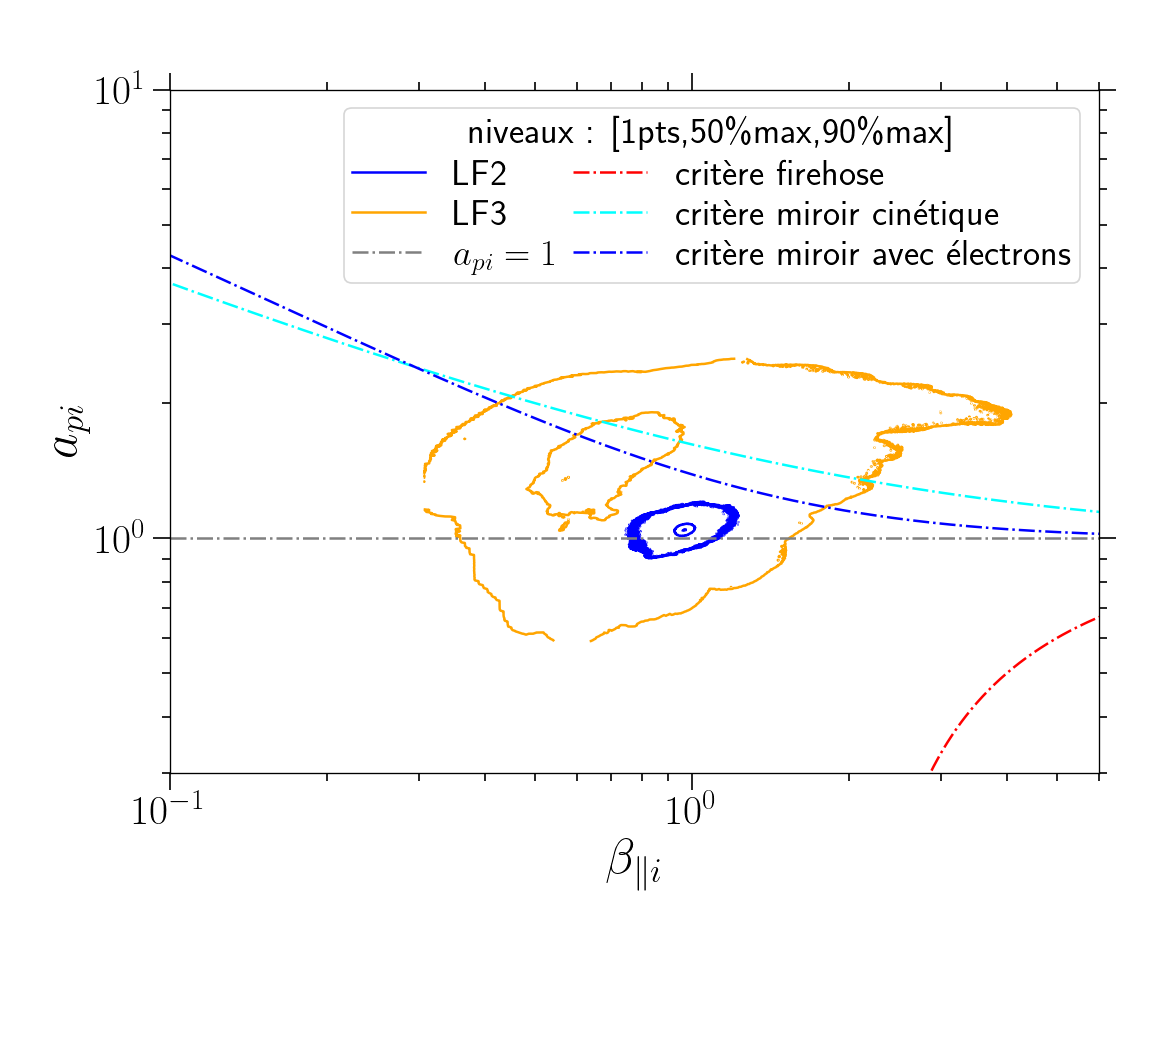
\includegraphics[width=1\linewidth,trim=0cm 2cm 1cm 1cm, clip=true]{./Part_3/images_ch4/diag_simu_LF}
\cprotect\caption{Diagramme $a_{pi}-\beta_{\parallel i}$ contenant l'histogramme \acs{2D} des simulations LF2 et LF3 sous la forme de courbes de niveau centrées sur le couple moyen. Les lignes discontinues correspondent aux critères d'instabilité. Rouge : le critère firehose CGL calculé dans le chapitre \ref{ch-21} et valable dans les modèles cinétique [\cite{hunana_introductory_2019}], il ne prend pas en compte l'effet \acs{Hall}. Cyan : critère miroir cinétique (sans prise en compte de la pression électronique) [\cite{hunana_introductory_2019}]. Bleu : critère miroir proposé par \cite{kuznetsov_mirror_2012}, prenant en compte les électrons gyrotropes et calculé avec $a_{pe} = 1$ et $\beta_{\parallel e } = 1$.}
\label{fig:diag_simu_LF}
\end{figure} 

Les taux d'anisotropie initialisés à $\num{1}$ sont restés proches de 1 et sont moins étalées que ceux des simulations \acs{CGLHPe} CGL2 et CGL3. LF3 montre un étalement plus important similairement à CGL3. Plus d'un tiers des points sont situés dans la zone du diagramme située du côté instable du critère miroir. Deux critères miroirs sont donnés. Le premier en cyan correspond au critère cinétique obtenue en corrigeant le facteur 6 du critère CGL [\cite{galeev_mhd_1983,ferriere_mixed_2002,hunana_introductory_2019}]. Le second, en bleu, est aussi un critère miroir cinétique mais prenant en compte l'anisotropie de pression électronique. Ce critère est dérivé dans l'article [\cite{kuznetsov_mirror_2012}]. Il est ici représenté en considérant $a_{pe} = 1$ et $\beta_{\parallel e } = 1$. 

Les simulations LF pourrait donc permettre une étude fine de l'impact des instabilités cinétiques sur la cascade turbulente. Mais, en première application de la loi exacte étendue et par curiosité, nous avons d'abord cherché à retrouver les résultats de \ac{F21}. 



\section{Premières applications de la loi exacte \acs{LFHPe}}
\label{sec-343}

Pour les simulations LF2 et LF3, l'extraction d'échantillons de temps consécutifs n'a pas encore été fait. On ne fera donc pas apparaître le niveau $\zeta$ dans les résultats qui suivent qui sont préliminaires.

L'une des questions que nous nous sommes posés est : est-ce que l'on retrouve la décroissance associée au flux de chaleur par \ac{F21} ? On a alors calculé le taux de cascade total dans LF2 et LF3 avec ($\varepsilon|\nabla \cdot \boldsymbol{q} \neq 0$) et sans ($\varepsilon|\nabla \cdot \boldsymbol{q} = 0$) la contribution du flux de chaleur. Les résultats sont montrés sur la figure \figref{fig:LF_q}.
\begin{figure}[!ht]
 \centering
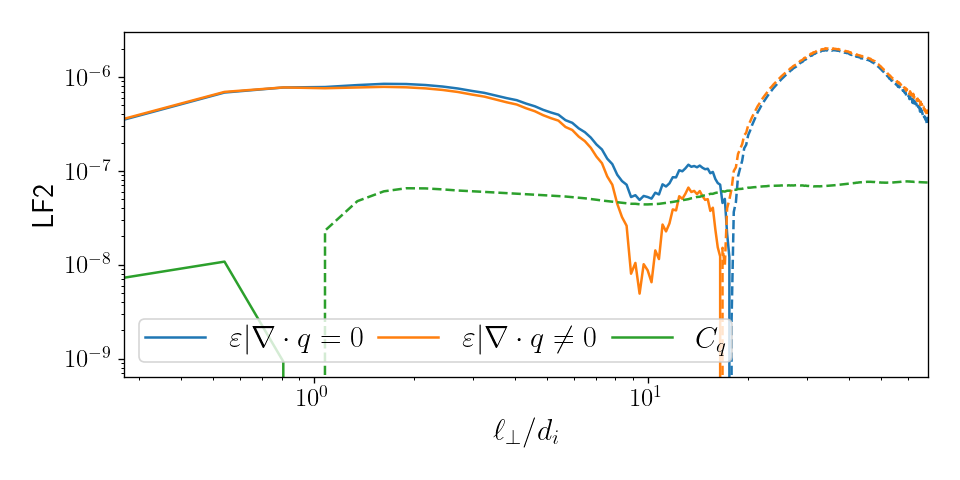
\includegraphics[width=0.9\linewidth,trim=1cm 1cm 0cm 1cm, clip=true]{./Part_3/images_ch4/LF2_q}
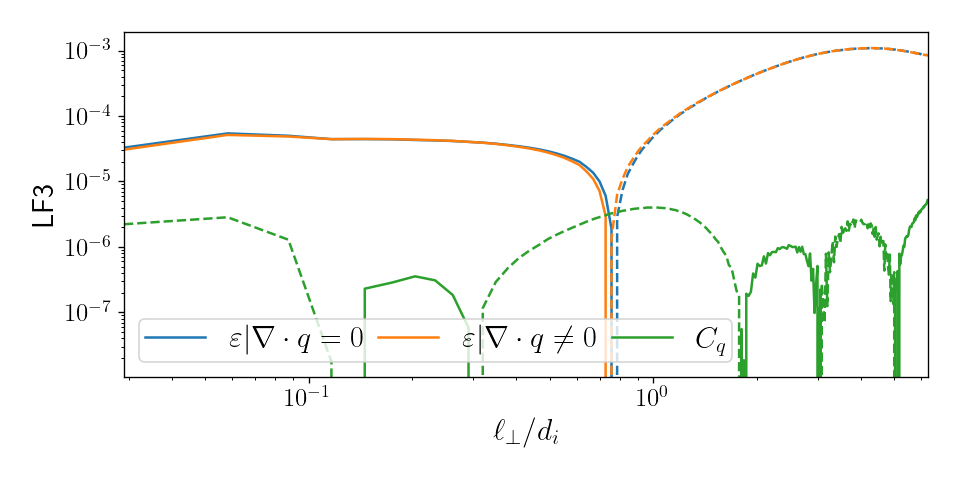
\includegraphics[width=0.9\linewidth,trim=1cm 1cm 0cm 1cm, clip=true]{./Part_3/images_ch4/LF3_q}
\cprotect\caption{Taux de cascade calculé en prenant en compte la contribution de flux de chaleur et en l'omettant.}
\label{fig:LF_q}
\end{figure} 
On remarque que la contribution du flux de chaleur ($C_q$, vert) semble négligeable même aux plus petites échelles. On ne retrouve donc pas la décroissance observée en allant vers les petites échelles que l'on s'attendait à voir en ne le prenant pas en compte en accord avec les résultats de \ac{F21}.

Afin de vérifier si une erreur ne s'était pas introduite dans notre calcul. Nous avons calculé la loi exacte la plus proche de la loi incompressible observée par \cite{ferrand_fluid_2021}, c'est-à-dire la loi Hall-MHD (HMHD) en n'y prenant en compte que les contributions isotropes des tenseurs de pression ionique et électronique, les termes dépendant de l'anisotropie de pression, du terme \acs{Pe} de la loi d'Ohm ou des flux de chaleur étant nouveaux dans l'estimation du taux de cascade. Ce taux de cascade est représenté en orange sur la figure \figref{fig:LF_detail}. On retrouve bien le résultat de \ac{F21} avec la décroissance en allant vers les petites échelles. Ayant deux résultats semblant en contradiction, $\varepsilon|\nabla \cdot \boldsymbol{q}$ (bleu) et $\varepsilon_{HMHD}$, j'ai ajouté une à une les nouvelles contributions afin de comprendre ce qu'il se passait. 

\begin{figure}[!ht]
 \centering
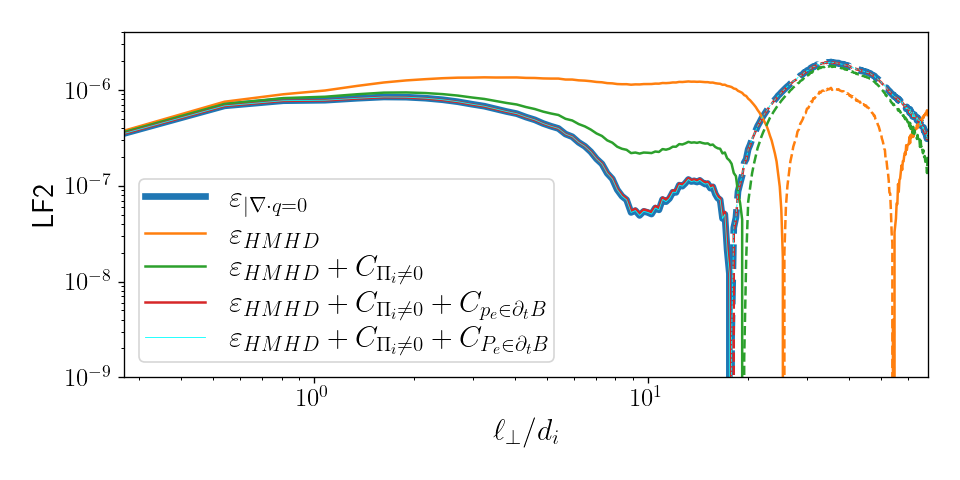
\includegraphics[width=1\linewidth,trim=1cm 1cm 0cm 1cm, clip=true]{./Part_3/images_ch4/LF2_detail}
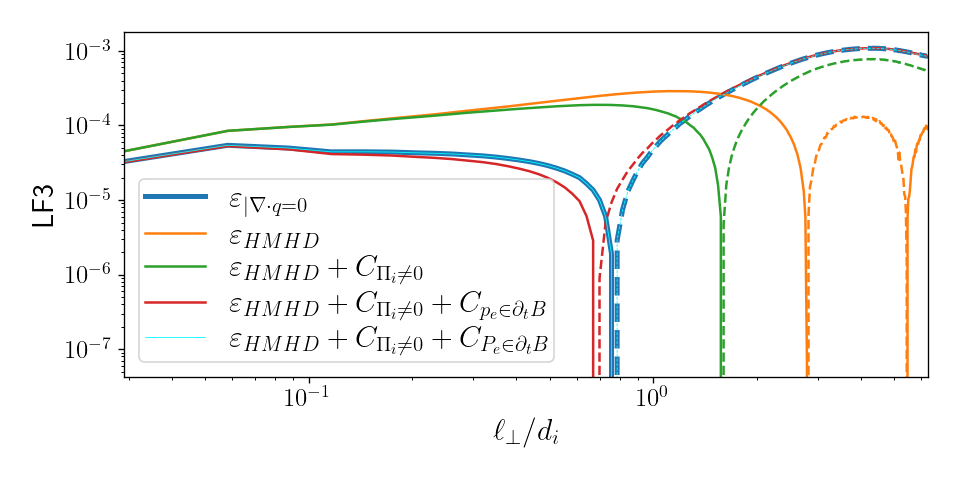
\includegraphics[width=1\linewidth,trim=1cm 1cm 0cm 1cm, clip=true]{./Part_3/images_ch4/LF3_detail}
\cprotect\caption{Taux de cascade calculé en prenant petit à petit en comptes les nouvelles contributions afin d'identifier quelles contributions impactent le taux de cascade \acs{LFHPe}. Le but étant de retrouver le taux de transfert  non linéaire total de ces simulations (courbe bleue épaisse) en partant d'une loi \acs{MHDH} (orange). Etape 1 (vert) : ajout de l'anisotropie de pression ionique. Etape 2 (rouge) : ajout de la contribution de pression électronique isotrope. Etape 3 (cyan) : prise en compte des anisotropies de pression électronique. Le taux de référence est quasiment retrouvé en ajoutant l'anisotropie de pression ionique et la pression isotrope électronique.}
\label{fig:LF_detail}
\end{figure} 
 Tout d'abord, on prend en compte l'anisotropie de pression des ions et des électrons (en gardant une loi d'Ohm Hall-MHD), le résultat correspond à la courbe verte. Le niveau du taux de cascade commence à s'affaisser aux échelles a priori inertielles, et à augmenter dans les échelles d'injections. Ces ajouts sont dominés par la pression ionique.

Ensuite, on ajoute la contribution de la pression électronique isotrope associée au terme \acs{Pe} de la loi d'Ohm, cela donne la courbe rouge. Le résultat est alors très proche du résultat voulu. La composante anisotrope des tenseurs de pression dans ce terme (résultat cyan) s'avère faible pour LF2 et influe un peu plus pour LF3. Le résultat  $\varepsilon|\nabla \cdot \boldsymbol{q}$ observé sur la \figref{fig:LF_q}
est ainsi retrouvé.

Ce résultat semble paradoxal face aux conclusions de \ac{F21}. Dans cet article, ils concluent en comblant la décroissance du taux de cascade par une estimation d'un taux de dissipation dû à l'amortissement Landau, remontant ainsi le niveau du taux de cascade dans la zone inertielle. De notre côté, on observe plutôt un affaissement du niveau du taux dû à la prise en compte de l'anisotropie de pression ionique ainsi que du tenseur de pression électronique dans l'équation d'induction. Ces résultats obtenus très récemment semblent venir questionner la méthode d'obtention du taux de dissipation par effet Landau utilisée par \ac{F21} ou notre interprétation de la contribution du flux de chaleur dans le taux de cascade et demande une analyse plus fine que ce qui a pu être fait jusqu'à présent. 

